\section{Introduction}
\vspace{0.2in}
\hspace*{0.16in}
In our case study, and from multiple articles, we can see that U-Net and Segnet models are dominating the field of cell segmentation.
In this chapter, we test out both U-Net and Segnet models, and analyse the results by comparing the two architectures.
We will also explore different machine learning algorithms for both preprocessing and postprocessing.

\section{Our approach}
\vspace{0.2in}
\hspace*{0.16in}
From all of the intel we have gathered, and previously read articles, all of cell segmentation (blood cell segmentation in particular) are mostly using U-Net and Segnet archtectures for segmenting blood cell images.
We have implemented both the U-Net and Segnet models.
In the following sections, a brief study analyzing and comparing both models with their perspective results.

\section{U-Net}
\subsection{Definition}
\lipsum[2-2]

\section{Segnet}
\subsection{Definition}
The SegNet neural network, developed by Alex Kendall, Vijay Badrinarayanan, and Roberto Cipolla, all from the University of Cambridge, is a convolutional neural network used for semantic pixel wise labeling. This problem is more commonly called semantic segmentation. \textsuperscript{\cite{badrinarayanan2017segnet}}

\subsection{Architecture}
SegNet has an encoder network and a corresponding decoder network, followed by a final pixelwise classification layer. This architecture is illustrated in the below figure.
With 13 encoder layers obtained from the VGG16 network, and 13 decoder layers to match the same number of encoder layers. The final decoder output is fed to a multi-class soft-max classifier to produce class probabilities for each pixel independently (pixelwise).

Each encoder in the encoder network performs convolution with a filter bank to produce a set of feature maps. These are then batch normalized. Then an element-wise rectified- linear non-linearity (ReLU) max(0, x) is applied. Following that, max-pooling with a 2x2 window and stride 2 (non-overlapping window) is performed and the resulting output is sub-sampled by a factor of 2. Max-pooling is used to achieve translation invariance over small spatial shifts in the input image.

The appropriate decoder in the decoder network upsamples its input feature map(s) using the memorized max-pooling indices from the corresponding encoder feature map(s). This step pro- duces sparse feature map(s). This SegNet decoding technique is illustrated in the below figure.
These feature maps are then convolved with a trainable decoder filter bank to produce dense feature maps. A batch normalization step is then applied to each of these maps. Note that the decoder corresponding to the first encoder (closest to the input image) produces a multi-channel feature map, although its encoder input has 3 channels (RGB).
This is unlike the other decoders in the network which produces feature maps with the same number of size and channels as their encoder inputs. The high dimensional feature representation at the output of the final decoder is fed to a trainable soft-max classifier.
This soft-max classifies each pixel independently. The output of the soft-max classifier is a K channel image of probabilities where K is the number of classes. The predicted segmentation corresponds to the class with maximum probability at each pixel. \textsuperscript{\cite{badrinarayanan2017segnet}}

\vspace{0.2in}

\begin{figure}[H]
\centering
  \vspace{-0.1in}
    \centerline{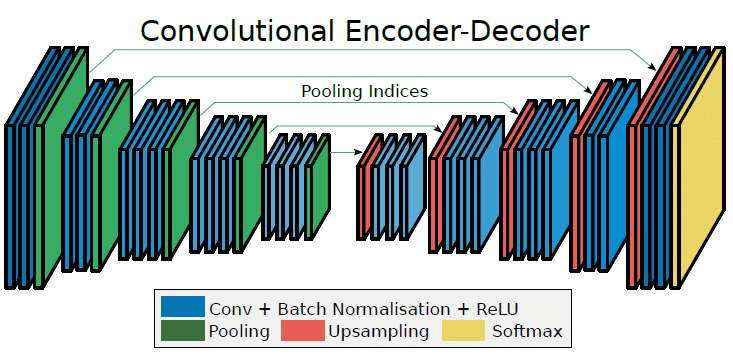
\includegraphics[width = 4in, height = 2.2in]{../images/segnet.png}}
    \caption{SegNet architecture}
\end{figure}

\subsection{Dataset}
For the segnet model, we have decided to test th ALL-IDB1 dataset, which contains 108 blood cell images, of which 10 images with their perspective masks and edge masks were chosen for red blood cell training and 3 as a test dataset, for white blood cells 73 images with their masks, and 33 as a test dataset.
For platelets, we used 71 for training and 31 as a test dataset.
Only red blood cells have edge masks, because we need to get rid of overlapped cells, white blood cells and platelets dont need the edge masks, using masks only can retrieve all the necessary features, because both white blood cells and platelets rarely overlap.
The images will be sliced and rescaled to 128x128 to match the input shape of the Segnet model.
The resulting train dataset will be 3916 image, mask, and edge tiles (a total of 11748 tiles).
For the test dataset 1072 image, mask, and edge tiles (a total of 3216 tiles) for red blood cells.
As for white blood cells, 28126 image and mask tiles were used for training (a total of 56252 tiles), and 15892 image and mask tiles were used as a test dataset for white blood cells (a total of 31784 tiles).
Finally, for platelets we used 27650 image and mask tiles were used for training (a total of 55300), and 14410 image and mask tiles as a test dataset for platelets (a total of 28820).

\vspace{0.1in}

% Please add the following required packages to your document preamble:
% \usepackage{multirow}
% \usepackage{graphicx}
% \usepackage[table,xcdraw]{xcolor}
% If you use beamer only pass "xcolor=table" option, i.e. \documentclass[xcolor=table]{beamer}
\begin{table}[H]
\centering
\resizebox{\textwidth}{!}{%
\begin{tabular}{|cc|c|c|c|c|c|c|}
\hline
\multicolumn{2}{|c|}{{\color[HTML]{000000} \textbf{Dataset}}}                                                                     & {\color[HTML]{000000} \textbf{\begin{tabular}[c]{@{}c@{}}Train\\ images\end{tabular}}} & {\color[HTML]{000000} \textbf{\begin{tabular}[c]{@{}c@{}}Test\\ images\end{tabular}}} & {\color[HTML]{000000} \textbf{\begin{tabular}[c]{@{}c@{}}Train\\ Tiles\end{tabular}}} & {\color[HTML]{000000} \textbf{\begin{tabular}[c]{@{}c@{}}Test\\ Tiles\end{tabular}}} & {\color[HTML]{000000} \textbf{\begin{tabular}[c]{@{}c@{}}Total\\ images\end{tabular}}} & {\color[HTML]{000000} \textbf{\begin{tabular}[c]{@{}c@{}}Total\\ tiles\end{tabular}}} \\ \hline
\multicolumn{1}{|c|}{{\color[HTML]{000000} }}                                             & {\color[HTML]{000000} \textbf{Image}} & {\color[HTML]{000000} 10}                                                              & {\color[HTML]{000000} 3}                                                              & {\color[HTML]{000000} 3916}                                                           & {\color[HTML]{000000} 1072}                                                          & {\color[HTML]{000000} 13}                                                              & {\color[HTML]{000000} \textbf{4988}}                                                  \\ \cline{2-8} 
\multicolumn{1}{|c|}{{\color[HTML]{000000} }}                                             & {\color[HTML]{000000} \textbf{Mask}}  & {\color[HTML]{000000} 10}                                                              & {\color[HTML]{000000} 3}                                                              & {\color[HTML]{000000} 3916}                                                           & {\color[HTML]{000000} 1072}                                                          & {\color[HTML]{000000} 13}                                                              & {\color[HTML]{000000} \textbf{4988}}                                                  \\ \cline{2-8} 
\multicolumn{1}{|c|}{\multirow{-3}{*}{{\color[HTML]{000000} \textbf{Red Blood Cells}}}}   & {\color[HTML]{000000} \textbf{Edge}}  & {\color[HTML]{000000} 10}                                                              & {\color[HTML]{000000} 3}                                                              & {\color[HTML]{000000} 3916}                                                           & {\color[HTML]{000000} 1072}                                                          & {\color[HTML]{000000} 13}                                                              & {\color[HTML]{000000} \textbf{4988}}                                                  \\ \hline
\multicolumn{1}{|c|}{{\color[HTML]{000000} }}                                             & {\color[HTML]{000000} \textbf{Image}} & {\color[HTML]{000000} 73}                                                              & {\color[HTML]{000000} 33}                                                             & {\color[HTML]{000000} 28126}                                                          & {\color[HTML]{000000} 15892}                                                         & {\color[HTML]{000000} 106}                                                             & {\color[HTML]{000000} \textbf{44018}}                                                 \\ \cline{2-8} 
\multicolumn{1}{|c|}{\multirow{-2}{*}{{\color[HTML]{000000} \textbf{White Blood Cells}}}} & {\color[HTML]{000000} \textbf{Mask}}  & {\color[HTML]{000000} 73}                                                              & {\color[HTML]{000000} 33}                                                             & {\color[HTML]{000000} 28126}                                                          & {\color[HTML]{000000} 15892}                                                         & {\color[HTML]{000000} 106}                                                             & {\color[HTML]{000000} \textbf{44018}}                                                 \\ \hline
\multicolumn{1}{|c|}{{\color[HTML]{000000} }}                                             & {\color[HTML]{000000} \textbf{Image}} & {\color[HTML]{000000} 71}                                                              & {\color[HTML]{000000} 31}                                                             & {\color[HTML]{000000} 27650}                                                          & {\color[HTML]{000000} 14410}                                                         & {\color[HTML]{000000} 102}                                                             & {\color[HTML]{000000} \textbf{42060}}                                                 \\ \cline{2-8} 
\multicolumn{1}{|c|}{\multirow{-2}{*}{{\color[HTML]{000000} \textbf{Platelets}}}}         & {\color[HTML]{000000} \textbf{Mask}}  & {\color[HTML]{000000} 71}                                                              & {\color[HTML]{000000} 31}                                                             & {\color[HTML]{000000} 27650}                                                          & {\color[HTML]{000000} 14410}                                                         & {\color[HTML]{000000} 102}                                                             & {\color[HTML]{000000} \textbf{42060}}                                                 \\ \hline
\end{tabular}%
}
\caption{Dataset used for segnet}
\label{Dataset used for segnet}
\end{table}


\subsection{Dataset augmentation}
We used the same dataset augmention on all cells (red, white blood cells, and platelets).
The augmentation we used was custom which involves the following steps:
\begin{enumerate}
    \item Pick a random image from the train dataset.
    \item Get the x and y coordinates randomly from the chosen image.
    \item Rescale the image randomly.
    \item Find the edges of a box around the image chip and the mask chip.
    \item Take a slice of the image and mask accordingly.
    \item Skip empty image chips (masks, and edge chips for red blood cells).
    \item Resize the image and mask chip to 128x128.
    \item Randomly rotate and flip the image chip.
    \item Randomly augment the colors (luminosity and saturation).
    \item Rescale the chip back to normal.
\end{enumerate}

\newpage
